\documentclass[tikz,border=6pt]{standalone}
\usepackage{amsmath,amssymb}
\usepackage{xcolor}
\definecolor{accent}{HTML}{A13D2C}
\definecolor{accent2}{HTML}{2B5F6B}
\definecolor{muted}{HTML}{5A564F}
\definecolor{panel}{HTML}{F8F6F0}
\definecolor{linecol}{HTML}{D8D2C4}
\definecolor{astroblue}{HTML}{1B4F72}
\definecolor{sunyellow}{HTML}{E8A33D}
\definecolor{colthree}{RGB}{60,140,80}
\usetikzlibrary{calc,arrows.meta,plotmarks}
\IfFileExists{results/ch12/lane_emden_n3.dat}{\def\datadir{results/ch12/}}{\def\datadir{../results/ch12/}}
\begin{document}
% Gamow peak for p + p at the Sun's centre: kT = 1.353 keV, E_G = 493 keV. Each curve is scaled to a maximum of 1:
%  Maxwell tail exp(-E/kT), tunnelling exp(-sqrt(E_G/E)) scaled to 1 at E = 20 keV, and their product.
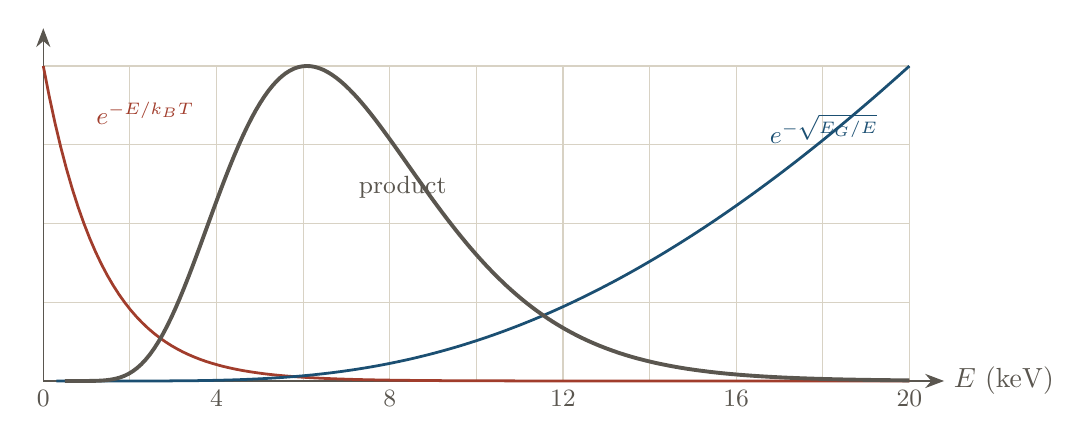
\begin{tikzpicture}[x=0.55cm,y=4cm, >={Stealth[length=2.4mm]}]
  \def\kT{1.353}\def\EG{493}
  \draw[linecol] (0,0) grid[xstep=2,ystep=0.25] (20,1);
  \draw[->, muted] (0,0) -- (20.8,0) node[right] {$E\ (\mathrm{keV})$};
  \draw[->, muted] (0,0) -- (0,1.12);
  \foreach \x in {0,4,8,12,16,20} \node[below, muted] at (\x,0) {\small \x};
  \draw[accent, line width=1.0pt, domain=0:20, samples=150] plot (\x, {exp(-\x/\kT)});
  \draw[astroblue, line width=1.0pt, domain=0.3:20, samples=150] plot (\x, {exp(-sqrt(\EG/\x)+sqrt(\EG/20))});
  \draw[muted, line width=1.4pt, domain=0.5:20, samples=200] plot (\x, {exp(-\x/\kT - sqrt(\EG/\x) + 6.088/\kT + sqrt(\EG/6.088))});
  \node[accent, right] at (1.0,0.85) {\small $e^{-E/k_BT}$};
  \node[astroblue, left] at (19.5,0.8) {\small $e^{-\sqrt{E_G/E}}$};
  \node[muted, above] at (8.3,0.55) {\small product};
\end{tikzpicture}
\end{document}
